\documentclass[12pt]{article}
\usepackage{amsmath}
\usepackage{graphicx,psfrag,epsf}
\usepackage{enumerate}
\usepackage{natbib}
\usepackage{url} % not crucial - just used below for the URL 
\usepackage{multirow}
\usepackage{caption}
\usepackage{mathtools}
\usepackage{amsfonts}
\usepackage{booktabs}
%\usepackage{graphicx}
\usepackage{soul}
\usepackage{color}
\usepackage{xspace}
\usepackage{subcaption}
\usepackage{amsmath}
\usepackage{algorithm}
\usepackage{algpseudocode}
\usepackage{mathtools}
\usepackage{xcolor}
\usepackage{url}
\usepackage{pifont}
\usepackage{hyperref}
\usepackage[section]{placeins}
\newcommand{\xmark}{\ding{55}}
% \usepackage[pdftex]{graphicx}
%\pdfminorversion=4
% NOTE: To produce blinded version, replace "0" with "1" below.
\newcommand{\blind}{0}

% DON'T change margins - should be 1 inch all around.
\addtolength{\oddsidemargin}{-.5in}%
\addtolength{\evensidemargin}{-.5in}%
\addtolength{\textwidth}{1in}%
\addtolength{\textheight}{.8in}%
\addtolength{\topmargin}{-1in}%


\begin{document}
{\fontsize{2.5}{4}\selectfont}
%\bibliographystyle{natbib}

% \def\spacingset#1{\renewcommand{\baselinestretch}%
% {#1}\small\normalsize} \spacingset{1}


%%%%%%%%%%%%%%%%%%%%%%%%%%%%%%%%%%%%%%%%%%%%%%%%%%%%%%%%%%%%%%%%%%%%%%%%%%%%%%

\if0\blind
{
  \title{\bf 
 Summary of SCAN: Learning to Classify Images without Labels
}
  \author{Rakibuzzaman Mahmud: 1141444{}\\
    Master Seminar: Deep Learning in Computer Vision\\
}
  \maketitle
} \fi

\if1\blind
{
  \bigskip
  \bigskip
  \bigskip
  \begin{center}
    {\LARGE\bf Title}
\end{center}
  \medskip
} \fi

 \renewcommand{\abstractname}{Overview}

\bigskip
\begin{abstract}

Convolutional neural networks have made breakthroughs in processing image, video, speech, and text and have recently been substantially improving upon the state of the art in image classification. But CNN often achieves their strong performance through supervised learning, which requires a huge amount of labeled dataset. But when there are no labels to train a network how do we get the network to learn meaningful features from the images? 

Combining representation learning with clustering is one of the most promising approaches for unsupervised learning.  The method described in the paper called SCAN(Semantic Clustering by Adopting Nearest neighbors) decouples the feature representation part and the clustering part resulting in a state of the art accuracy. The authors try to solve the problem with 3 steps: 
Self Supervised Learning: a self-supervised task from representation learning tries to extract semantically meaningful features. Clustering: clustering the similar representation using Nearest-neighbor-based Clustering. Self Labelling: using already well-classified images and fixing mistakes through self-labeling. SCAN method is the first to perform well on a large-scale dataset for image classification and shows promising results on ImageNet. Furthermore, it outperforms several semi-supervised learning methods with unlabelled data.

\end{abstract}

\noindent%
{\it Keywords:} Unsupervised Learning, Self-Supervised Learning, Image
Classification, Clustering.
\vfill

\newpage

% \spacingset{1.45} % DON'T change the spacing!

\section{Introduction}
\label{sec:intro}
A conventional image classification task involves labels that govern the features it learns through a Loss function. Humans are better at detecting objects where CNN's use supervised learning algorithms that require a huge amount of labeled images. However, acquiring labeled data or manually labeling data is often an expensive process and in the real-world scenario labeled data are hard to come by.

\medskip
There are many approaches to solve this problem such as semi-supervised, self-supervised
\cite{DeepMetricLearning} 
semi-supervised learning is the branch of machine learning concerned with using labeled as well as unlabelled data to perform certain learning tasks. But they still require some amount of labeled data to get better performance. However, a major question remains. How can we classify images when there are no ground-truths available during the training or what if we do not know how many classes are there to classify?

\medskip

To address these questions researchers have been trying to use unsupervised learning methods.\cite{xie2016unsupervised} The goal of this approach is to cluster similar images together, while images in different clusters are dissimilar. Applying clustering algorithms to images is a difficult task. For instance, consider two images of dogs, one black and one white. The different pixel values cannot be directly clustered. So we need a feature selector. But Hand-engineered features are quite tedious to produce and do not perform that well in practice. 
Self-supervised learning such as Representation learning \cite{doersch2016unsupervised}\cite{gidaris2018unsupervised} can be used to generate feature representations from images. When we have a better representation of an image, we can cluster them using a loss function. But this approach will tend to focus on low-level features and we can not be sure if this will be semantically meaningful.  

\medskip
The method described in the paper separates the feature representation and the clustering resulting in inaccuracy almost as similar to the supervised method. Also, to further improve results the authors applied Fine-Tuning through self-labeling. The authors of the paper also observed, depending on the K value, sometimes semantically different images were clustered together. To address this issue, images that had a probability of belonging to a cluster were selected and labeled and these labeled images were used with their neighbors to update the weights and Cross entropy loss that optimizes those data points. Which as a result, makes the predictions more accurate. 

% \begin{figure}
% \begin{center}
% \includegraphics[width=3in]{fig1.pdf}
% \end{center}
% \caption{Consistency comparison in fitting surrogate model in the tidal
% power example. \label{fig:first}}
% \end{figure}

\newpage


\section{Related work}

\bigskip


This paper relates to many broad areas of research: The major topics that are covered in the paper are briefly discussed below.




\subsection{Convolutional Neural Network}
% \label{sec:2}

The Convolutional Neural Network (CNN) uses deep learning architecture inspired by the visual perception system of the living creatures.
\cite{hubel1968receptive}

\bigskip
The basic components of a CNN consist of three types of layers, convolutional layer, pooling layer, and fully-connected layer. 
The convolutional layer learns feature representations of image data. 
The pooling layer aims to preserve the detected features in a smaller representation by discarding less significant data at the cost of spatial resolution. A CNN may consist of multiple convolutional and pooling layers and they are connected with one or more fully-connected layers that aim to perform high-level reasoning [11]. They take all neurons in the previous layer, connect them to every single neuron of the current layer to generate semantic information.\cite{zeiler2014visualizing}

\medskip

CNN's have been applied in image classification for a long time.\cite{zuo2015exemplar,nogueira2017towards} With their better capability of joint feature and classifier learning
CNN's can achieve better classification accuracy on large scale datasets 
Compared to the other methods.\cite{simonyan2014very} A point to be noted that, all the best results are coming from supervised training using labeled data. However, these labeled data are not easy to collect. Furthermore, these systems are difficult to scale up and can not handle many types of fine-grained classes. To solve this problem, some researchers propose to find localized regions in an unsupervised manner.\cite{xie2016unsupervised}


\subsection{Self-supervised representation learning}  

Self-supervised learning is a subset of unsupervised learning methods, in which CNN is explicitly trained with automatically generated labels. 

\medskip

Since The labels are automatically generated during self-supervised training large-scale datasets can be used for self-supervised training. Trained with these generated labels, self-supervised methods achieve promising results, and the gap between supervised methods and self-supervised learning methods are getting closer with new researches.\cite{jing2020self}

\medskip

Representation learning is a set of techniques that allows a system to automatically discover the representations needed for feature detection or classification from image data.
A wide variety of representation learning methods have been proposed for the self-training of deep convolutional neural networks. 



These methods use various pre-designed tasks called pretext tasks, which do not require annotated data to learn the representation and they are applied in-painting \cite{pathak2016context}, patch context and jigsaw puzzles \cite{doersch2016unsupervised}; \cite{noroozi2017unsupervised}; \cite{noroozi2018boosting}, clustering \cite{caron2019deep}; \cite{zhuang2019selfsupervised} colorization \cite{zhang2016colorful},
generation \cite{jenni2018selfsupervised}; \cite{donahue2019large}, predicting transformations \cite{gidaris2018unsupervised}; \cite{zhang2019aet} and  predicting rotation\cite{gidaris2018unsupervised}.

\bigskip

But still, they have not managed to match the performance of supervised-learned representations, but they have proved to be good alternatives for transferring on other vision tasks, such as object recognition, object detection, and semantic segmentation. 





\subsection{Data Clustering} 

Much research has been devoted to data clustering methods. We can primarily divide the existing methods into three categories: distance-based, density-based, and connectivity-based methods.  \cite{madhulatha2012overview}

Distance-based methods, such as the K-means \cite{jin2010k}, seek to find the relationship between data points based on various distance metrics. Density-based methods attempt to cluster data points via a proper density function, including the density-based spatial clustering of applications with noise.\cite{inbook} Compared with the previous methods, connectivity-based methods cluster data points into a cluster if they are highly connected. \cite{LEE2021107708}



\subsection{Combination of Feature learning and Clustering} 

Recently, several methods have been proposed to combine feature learning with clustering into a single model. Such as deep embedded clustering (DEC)\cite{xie2016unsupervised} which is a method that simultaneously learns feature representations and cluster assignments using deep neural networks. DEC learns a mapping from the data space to a lower-dimensional feature space in which it iteratively optimizes a clustering objective. 

\medskip

There are also other methods i.e: DAC \cite{chang2017deep} which leverages the architecture of CNNs for image clustering. Additionally, Another clustering method  DeepCluster  \cite{caron2018deep} that jointly learns the parameters of a neural network and the cluster assignments of the resulting features. DeepCluster iteratively groups the features with a standard clustering algorithm, k-means, and uses the subsequent assignments as supervision to update the weights of the network.





\newpage

\section{Method}
\label{sec:method}

The method of the paper can be described in a three step process:

\medskip

First, Producing semantically meaningful feature representations using a pretext task, which is done in a Self supervised manner. 

\medskip

Second, Classify each image and its nearest neighbors together using a novel loss function.

\medskip

Third, Using a self-labeling approach to reduce noise and make the clustering as close as possible to the class distribution of the k nearest neighbors in the neighbor selection. 

\subsection{Representation learning for semantic clustering and Pretext Task}


The paper uses representation learning as the  pretext task $\tau$, that learns an embedding function $\Phi_\theta$ - parameterized by a neural network with weights $\theta$ - that maps images into feature representations.

\begin{equation}
\label{eq:pretext_task}
    \min_{\theta}d(\Phi_\theta(X_i), \Phi_\theta(T[X_i])).
\end{equation}

The main idea behind this is that if we transform the images, whether it be cropping or changing contrast, the high level features should remain the same. 

\medskip

After  transforming the images and getting a new dataset of transformed images we use a convolution neural network to produce a feature representation of both the images and the transformed images and optimize the distance between the outputs for the image and the transformed image . When the original image and transformed image are in the same cluster with the objective of minimising the distance between $[X_i]$ and their augmentations $(T[X_i])$, the learned representations are much more meaningful.




\subsection{A semantic clustering loss} 

After getting a meaningful representation, we can apply K-means or any clustering algorithm to it . But naively applying K-means to get K clusters can lead to ‘cluster degeneracy’.

To solve this issue the paper introduces Semantic clustering loss, which aims to learn a clustering function $\Phi_\eta$ - parameterized by a neural network with weights $\eta$ which is able to classify a sample $X_i$ and its mined neighbors $\mathcal{N}_{X_i}$ together. 

The function $\Phi_\eta$ terminates in a softmax function to perform a soft assignment over the clusters $\mathcal{C}=\left\{1,\ldots,C\right\}$, with $\Phi_\eta \left(X_i\right) \in [0,1]^C$. The probability of sample $X_i$ being assigned to cluster $c$ is denoted as $\Phi_\eta^c(X_i)$. the weights of $\Phi_\eta$ are learned by minimizing the following objective:

\begin{equation}
\label{eq:loss_objective}
\begin{split}
\Lambda = -\frac{1}{|\mathcal{D}|}\sum\limits_{X\in\mathcal{D}}\sum\limits_{k\in\mathcal{N}_{X}}&\log\left<\Phi_\eta(X),\Phi_\eta(k)\right> + \lambda\sum_{c\in\mathcal{C}} \Phi_\eta'^c \log \Phi_\eta'^c, \\
&\text{with~} \Phi_\eta'^c = \frac{1}{|\mathcal{D}|}\sum\limits_{X\in\mathcal{D}}\Phi_\eta^c(X).
\end{split}
\end{equation}





The idea is to pass these images and its mined neighbors from the previous stage to a Neural Network to output probabilities for all the classes. The classes are chosen using some knowledge initially, the paper uses the knowledge of ground truth for the evaluation purposes.  


\medskip

The goal of the loss function is to make the clustering of an image as close as possible to the class distribution of the k nearest neighbors.
This is done by the dot product of the image vector of probabilities and its neighbor’s vector. 







\subsection{ Fine-tuning through self-labeling} 

After clustering, some of the data points do not belong to the same semantic cluster. These false-positive examples make uncertain predictions. Therefore, the authors used a self-labeling approach to correct for mistakes due to noisy nearest neighbors 
using the already well-classified examples  \cite{sohn2020fixmatch}. To be more specific, each sample was combined with K $\geq$ 1 neighbors, some of which unavoidably do not relate to the corresponding semantic cluster. These false-positive samples point to predictions for which the network is less confident.  At the same time, the authors inspected that examples with highly confident predictions tend to be classified into a proper cluster, and consequently, a self-labeling strategy can be used to utilize the already well-classified examples, and correct the errors due to noisy nearest neighbors.
 

\begin{algorithm}[H]
\small{
\caption{Semantic Clustering by Adopting Nearest neighbors (SCAN)}
\label{alg: algorithm}
\begin{algorithmic}
\State \textbf{Input:} Dataset $\mathcal{D}$, Clusters $\mathcal{C}$, Task $\tau$, Neural Nets $\Phi_\theta$ and $\Phi_\eta$, Neighbors $\mathcal{N}_\mathcal{D}=\{\}$.

\State Optimize $\Phi_\theta$ with task $\tau$ in Eq.~\ref{eq:pretext_task}. \Comment Pretext Task Step 
\For{$X_i \in \mathcal{D}$}
\State $\mathcal{N}_\mathcal{D} \leftarrow \mathcal{N}_{\mathcal{D}} \cup \mathcal{N}_{X_i}$, with $\mathcal{N}_{X_i} = K$ neighboring samples of $\Phi_\theta(X_i)$.
\EndFor
\While{SCAN-loss decreases} \Comment Clustering Step
\State Update $\Phi_\eta$ with SCAN-loss, i.e. $\Lambda(\Phi_\eta(\mathcal{D}), \mathcal{N}_{\mathcal{D}}, C)$ in Eq.~\ref{eq:loss_objective}
\EndWhile 

\While{$Len(Y)$ increases} \Comment Self-Labeling Step
\State Y $\leftarrow$ ($\Phi_\eta(\mathcal{D}) >$ threshold)   
\State Update $\Phi_\eta$ with cross-entropy loss, i.e. $H(\Phi_\eta(\mathcal{D}), Y)$
\EndWhile

\State \textbf{Return:} $\Phi_\eta(\mathcal{D})$ \Comment{$\mathcal{D}$ is divided over $C$ clusters}
\end{algorithmic}
}
\end{algorithm}

\newpage



\section{Experiments}
\label{sec:verify}


\subsection{Datasets}

The dataset that were considered for the experiments are  CIFAR10 \cite{CIFAR}, CIFAR100- 20 \cite{CIFAR} STL10 \cite{yao2016automatic} and ImageNet \cite{ImageNet}.

%
%\begin{figure}[!htbp]
%\begin{center}
%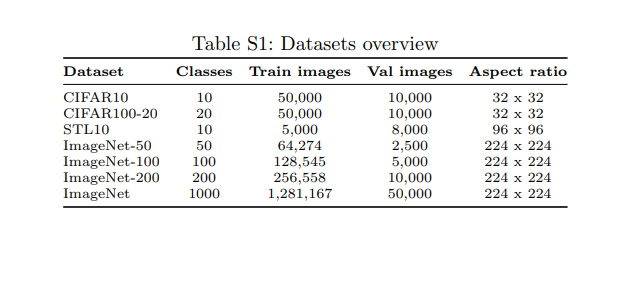
\includegraphics[width=6in]{6.PNG}
%\end{center}
%\end{figure}
%

%%%%%%%%%%%%%%%%%%%%%%%%%%%%%%%%%%

\setlength{\tabcolsep}{4pt}
\begin{table}[ht!]
\scriptsize
\begin{center}
\caption{Datasets overview}
\label{tab: datasets}
\begin{tabular}{@{}l cccc @{}}
\toprule
\textbf{Dataset} & \textbf{Classes} & \textbf{Train images} & \textbf{Val images} & \textbf{Aspect ratio}\\ 
\midrule
CIFAR10 & 10 & 50,000 & 10,000 & 32 x 32\\
CIFAR100-20 & 20 & 50,000 & 10,000 & 32 x 32\\
STL10 & 10 & 5,000 & 8,000 & 96 x 96\\
ImageNet-50 & 50 & 64,274 & 2,500 & 224 x 224\\
ImageNet-100 & 100 & 128,545 & 5,000 & 224 x 224\\
ImageNet-200 & 200 & 256,558 & 10,000 & 224 x 224\\
ImageNet & 1000 & 1,281,167 & 50,000 & 224 x 224\\
\bottomrule
\end{tabular}
\end{center}
\end{table}

%%%%%%%%%%%%%%%%%%%%%%%%%%%%%%%%%%

\subsection{Training setup}

The training was done on standard ResNet-18 backbone with batch size 128 and in the fine tuning step with threshold of 0.99 and using Adam optimizer. For every sample, the 20 nearest neighbors are determined through an instance discrimination task based on noise contrastive estimation (NCE) \cite{gutmann2010noise}  and SimCLR \cite{chen2020improved} implementation for the instance discrimination task on the dataset and MoCo \cite{chen2020simple} on ImageNet.


\subsection{Validation criterion} 

The model based on the lowest loss was selected as the best model during the clustering step.
For the self-labeling step, Based on the number of confident samples the model’s weights were saved.



\subsection{Augmentations} 

The authors were able to get better results using strong augmentations during the training. 
RandAugment \cite{cubuk2020randaugment}, followed by Cutout \cite{devries2017improved} for the augmentation part and it was composed of four randomly selected transformations.

\newpage

\subsection{Ablation studies} 
An ablation study studies the performance of an AI system by removing certain components, to understand the contribution of the component to the overall system. The term is by analogy with biology (removal of components of an organism), and, continuing the analogy, is particularly used in the analysis of artificial neural nets, by analogy with ablative brain surgery.\cite{DBLP:journals/corr/abs-1901-08644}



%%%% ABLATION METHOD TABLE %%%
%\setlength{\tabcolsep}{4pt}
%\begin{table}[t]
%\begin{minipage}[t]{0.5\linewidth}
%\scriptsize
%\begin{center}
%\caption{Ablation Method CIFAR10}
%\label{table:ablation_method}
%\begin{tabular}{lcc}
%\toprule
%\textbf{Setup} & \ \textbf{ACC} \\
% &  (Avg $\pm$ Std) \\
%\midrule
%Pretext + K-means & $65.9\pm5.7$ \\
%%Sample + Batch Entropy Loss & $19.2\pm0.9$ \\
%%SCAN-Loss (Standard Augs) (Ours)& $62.7\pm3.3$ \\
%SCAN-Loss (SimCLR) & $78.7\pm1.7$ \\
%\hspace{0.1in} (1) Self-Labeling (SimCLR) & $10.0\pm0$ \\
%\hspace{0.1in} (2) Self-Labeling (RA) & $87.4\pm1.6$ \\
%SCAN-Loss (RA) & $81.8\pm1.7$ \\
%\hspace{0.1in} (1) Self-Labeling (RA) & $87.6\pm0.4$ \\
%\bottomrule
%\end{tabular}
%\end{center}
%\end{minipage}
%\hspace*{\fill}
%\begin{minipage}[t]{0.5\linewidth}
%\scriptsize
%\begin{center}
%\caption{Ablation Pretext CIFAR10}
%\label{table: ablation_pretext}
%\begin{tabular}{lcc}
%\toprule
%\textbf{Pretext Task} & \textbf{Clustering}& \textbf{ACC}\\
%  & & (Avg $\pm$ Std)  \\
%\midrule
%RotNet~\cite{RotNet}  & K-means & $27.1\pm2.1$ \\
%  & SCAN & $74.3\pm3.9$ \\
%%Feature Decoupling~\cite{feng2019self} & $83.0\pm3.4$\\
%Inst. discr.~\cite{wu2018unsupervised} & K-means & $52.0\pm4.6$\\
% & SCAN &  $83.5\pm4.1$\\
%Inst. discr.~\cite{chen2020simple} & K-means & $65.9\pm5.7$ \\
% & SCAN &  $87.6\pm0.4$\\
%\bottomrule
%\end{tabular}
%\end{center}
%\end{minipage}
%\end{table}
%\setlength{\tabcolsep}{1.4pt}


%
\begin{figure}[!htbp]
\begin{center}
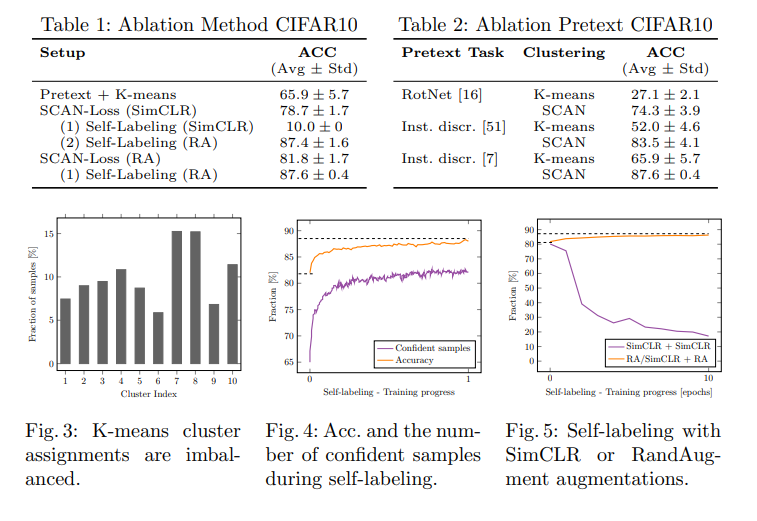
\includegraphics[width=6in]{8.PNG}
\end{center}
\end{figure}

\FloatBarrier

\medskip

The paper presented the performance gains through an ablation study on CIFAR10.



Some observation to be noted, K-means clustering with NCE pretext features results in an accuracy of 65.9\%. Interestingly, applying K-means to the pretext features outperforms prior state-of-the-art methods for unsupervised classification based on end-to-end learning schemes. This observation supports the paper's primary claim of the benefit of separating clustering and feature learning.

Applying image augmentation to both the samples and their mined neighbors also improves the performance (78.7\% vs. 81.8\%). During self-labeling, the network slowly becomes more confident and therefore fine-tuning the network enhances the quality of the clustering(81.8\% to 87.6\%). 



\newpage
\section{Comparison}
\label{sec:verify}


The Table below compares the result to the state-of-the-art on three different benchmarks clustering accuracy (ACC), normalized mutual information (NMI), and adjusted rand index (ARI). 


%
%\begin{figure}[!htbp]
%\begin{center}
%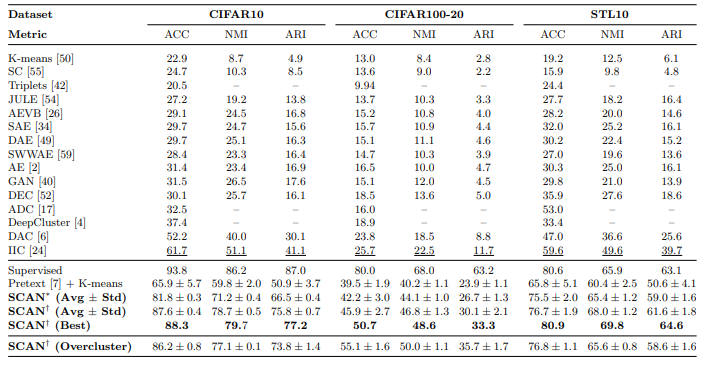
\includegraphics[width=6in]{3.PNG}
%\end{center}
%\caption{ \label{fig:first}}
%\end{figure}
%
%

%%% STATE-OF-THE-ART TABLE %%%%
\setlength{\tabcolsep}{4pt}
\begin{table}[ht]
\begin{center}
\label{table:sota}
\resizebox{\columnwidth}{!}{
\begin{tabular}{@{}l c ccc c ccc c ccc@{}}
\toprule
\textbf{Dataset} && \multicolumn{3}{c}{\textbf{CIFAR10}} && \multicolumn{3}{c}{\textbf{CIFAR100-20}} && \multicolumn{3}{c}{\textbf{STL10}} \\
\cmidrule{3-5} \cmidrule{7-9} \cmidrule{11-13}
\textbf{Metric} && ACC & NMI & ARI && ACC & NMI & ARI&& ACC & NMI & ARI \\
\midrule
\noalign{\smallskip}

K-means~\cite{wang2015optimized}     && 22.9 & 8.7   & 4.9  && 13.0  & 8.4  & 2.8 && 19.2 & 12.5 & 6.1  \\
Triplets~\cite{schultz2004learning}  && 20.5 & --    & --   && 9.94  & --   & --  && 24.4 & --   & --   \\
JULE~\cite{yang2016joint}            && 27.2 & 19.2  & 13.8 && 13.7  & 10.3 & 3.3 && 27.7 & 18.2 & 16.4 \\
AEVB~\cite{kingma2013auto}           && 29.1 & 24.5  & 16.8 && 15.2  & 10.8 & 4.0 && 28.2 & 20.0 & 14.6 \\
SAE~\cite{ng2011sparse}              && 29.7 & 24.7  & 15.6 && 15.7  & 10.9 & 4.4 && 32.0 & 25.2 & 16.1 \\
DAE~\cite{vincent2010stacked}        && 29.7 & 25.1  & 16.3 && 15.1  & 11.1 & 4.6 && 30.2 & 22.4 & 15.2 \\
SWWAE~\cite{zhao2015stacked}         && 28.4 & 23.3  & 16.4 && 14.7  & 10.3 & 3.9 && 27.0 & 19.6 & 13.6 \\
AE~\cite{bengio2007greedy}           && 31.4 & 23.4  & 16.9 && 16.5  & 10.0 & 4.7 && 30.3 & 25.0 & 16.1 \\
GAN~\cite{radford2015unsupervised}   && 31.5 & 26.5  & 17.6 && 15.1  & 12.0 & 4.5 && 29.8 & 21.0 & 13.9 \\
DEC~\cite{DEC}                       && 30.1 & 25.7  & 16.1 && 18.5  & 13.6 & 5.0 && 35.9 & 27.6 & 18.6 \\
ADC~\cite{haeusser2018associative}   && 32.5 & --    & --   && 16.0  & --   & --  && 53.0 & --   & --   \\
DeepCluster~\cite{DeepCluster}       && 37.4 & --    & --   && 18.9  & --   & --  && 33.4 & --   & --   \\
DAC~\cite{DAC}                       && 52.2 & 40.0 & 30.1 && 23.8& 18.5 & 8.8 && 47.0 & 36.6 & 25.6 \\
IIC~\cite{IIC} && \underline{61.7} & \underline{51.1}  & \underline{41.1} && \underline{25.7}  & \underline{22.5} & \underline{11.7}&& \underline{59.6} & \underline{49.6} & \underline{39.7} \\
%\textbf{SCAN$^\dagger$ (Ours)} && \textbf{88.6} & \textbf{80.3} & \textbf{77.9} && \textbf{50.5} & \textbf{47.4} & \textbf{32.8} && \textbf{81.2} & \textbf{70.1} & \textbf{65.1} \\
\midrule
Supervised  && 93.8 &  86.2 & 87.0   && 80.0 & 68.0 & 63.2 && 80.6 & 65.9 & 63.1\\
Pretext~\cite{chen2020simple} + K-means && $65.9\pm5.7$ & $59.8\pm2.0$ & $50.9\pm3.7$   && $39.5\pm1.9$ & $40.2\pm1.1$ & $23.9\pm1.1$ && $65.8\pm5.1$ & $60.4\pm2.5$ & $50.6\pm4.1$\\
\textbf{SCAN$^*$ (Avg $\pm$ Std) }  &&$81.8\pm0.3$ & $71.2\pm 0.4$ & $66.5\pm0.4 $&& $42.2\pm3.0$ & $44.1\pm1.0$ & $26.7\pm1.3$ && $75.5\pm2.0$ & $65.4\pm1.2$&$59.0\pm1.6$  \\
\textbf{SCAN$^\dagger$ (Avg $\pm$ Std) } &&$87.6\pm0.4$ & $78.7\pm 0.5$ & $75.8\pm0.7 $&& $45.9\pm2.7$ & $46.8\pm1.3$ & $30.1\pm2.1$ && $76.7\pm1.9$ & $68.0\pm1.2$&$61.6\pm1.8$  \\
\textbf{SCAN$^\dagger$ (Best)} && \textbf{88.3} &\textbf{79.}7 & \textbf{77.2} && \textbf{50.7} & \textbf{48.6} & \textbf{33.3} && \textbf{80.9} & \textbf{69.8} & \textbf{64.6} \\
\midrule
%\textbf{SCAN$^*$ (Overcluster)} &&$81.0\pm1.1$ & $70.3\pm1.0$ & $65.3\pm1.8 $&& $51.8\pm1.2$ & $47.3\pm0.9$ & $31.4\pm1.1$ && $76.8\pm1.1$ & $65.6\pm0.8$&$58.6\pm1.6$  \\
\textbf{SCAN$^\dagger$ (Overcluster)} &&$86.2\pm0.8$ & $77.1\pm 0.1$ & $73.8\pm1.4 $&& $55.1\pm1.6$ & $50.0\pm1.1$ & $35.7\pm1.7$ && $76.8\pm1.1$ & $65.6\pm0.8$&$58.6\pm1.6$  \\
\bottomrule
\end{tabular}
}
\end{center}

\caption{State-of-the-art comparison}
\end{table}
\setlength{\tabcolsep}{1.4pt}

\FloatBarrier
The proposed method consistently outperforms prior work by large margins on all three metrics, e.g. +26.6\% on CIFAR10, +25.0\% on CIFAR100-20 and +21.3\% on STL10 in terms of accuracy. 

\medskip


\subsection{ImageNet Experiments} 

To check the performance of the proposed SCAN method, the authors used the ImageNet dataset with smaller subsets of 50, 100, and 200 randomly selected classes that outperformed several semi-supervised learning methods without the use of any ground truth annotations. 
 

\begin{figure}[hbt!]
\begin{center}
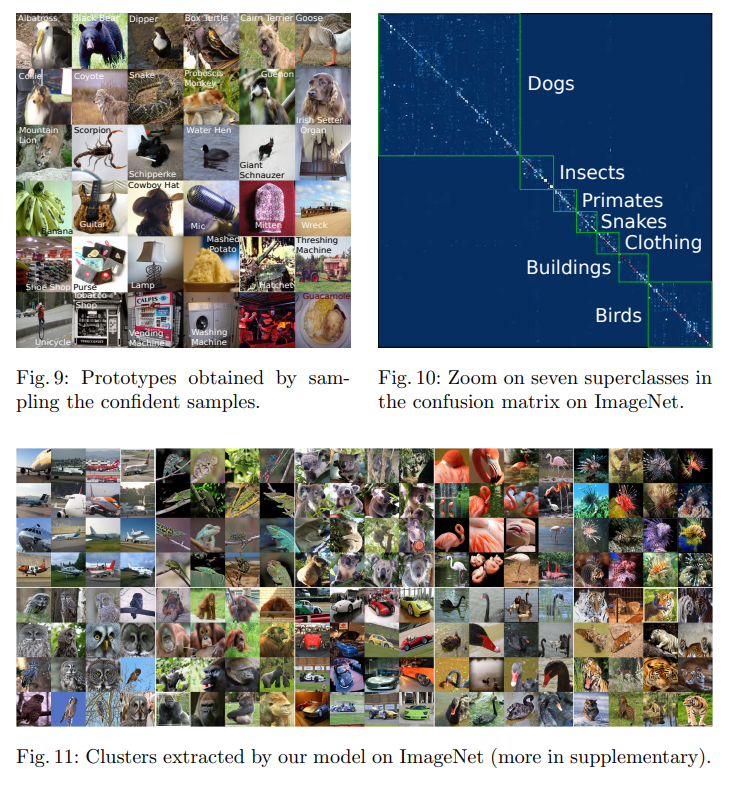
\includegraphics[width=6in]{7.PNG}
\end{center}
\end{figure}
Finally, the table also includes results that compare with the state-of-the-art in representation learning and when solving the problem in a fully-supervised manner. 


\FloatBarrier


\medskip

The Paper considers the problem of unsupervised image classification on the large-scale ImageNet dataset as shown in Table 3. First smaller subsets of 50, 100, and 200 randomly selected classes are considered and then the sets of 50 and 100 classes are subsets of the 100 and 200 classes respectively. 


%%% Imagenet TABLE %%%%
\setlength{\tabcolsep}{4pt}
\begin{table}[ht]
\begin{center}
\caption{Validation set results for 50, 100 and 200 randomly selected classes from ImageNet.}
\label{table: imagenet_subsets}
\resizebox{\columnwidth}{!}{
\begin{tabular}{@{}l c cccc c cccc c cccc@{}}
\toprule
\textbf{ImageNet} && \multicolumn{4}{c}{\textbf{50 Classes}} && \multicolumn{4}{c}{\textbf{100 Classes}} && \multicolumn{4}{c}{\textbf{200 Classes}} \\
\cmidrule{3-6} \cmidrule{8-11} \cmidrule{13-16}
\textbf{Metric} && Top-1 & Top-5 & NMI & ARI && Top-1 & Top-5 & NMI & ARI && Top-1 & Top-5 & NMI & ARI \\
\midrule
\noalign{\smallskip}
\textbf{K-means} && 65.9& - & 77.5 & 57.9 && 59.7 & - & 76.1 & 50.8 && 52.5& - & 75.5& 43.2 \\
\textbf{SCAN$^{*}$} && 75.1 & 91.9 & 80.5 & 63.5 && 66.2 & 88.1 & 78.7 & 54.4 && 56.3 & 80.3 & 75.7 & 44.1 \\
\textbf{SCAN$^{\dagger}$}  && 76.8 & 91.4 & 82.2 & 66.1 && 68.9 & 86.1 & 80.8 & 57.6 && 58.1 & 80.6 & 77.2 & 47.0 \\
\bottomrule
\end{tabular}
}
\end{center}

\end{table}
\setlength{\tabcolsep}{1.4pt}
 

\subsection{Overclustering}  

The network was trained with the knowledge of the number of ground-truth classes. However, the table 2 also reports the results when the number of clusters does not match the number of ground-truth classes. 

It can be observed that the approach does not require knowledge of the exact number of clusters and the increased performance on CIFAR100-20 is related to the higher intra-class variance. 

%\begin{figure}[!htbp]
%\begin{center}
%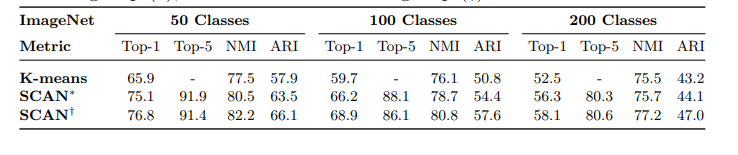
\includegraphics[width=6in]{4.PNG}
%\caption{Overclustering Figure}
%\end{center}
%\end{figure}





\section{Conclusion}
\label{sec:conc}


The approach described in this paper has produced state of the art results on a variety of datasets. 
But it comes with its own set of disadvantages. There are many hyperparameters to consider, like the number of clusters, the value of K or the transformation for self-supervised training. Also the algorithm performs less than optimally for large class sizes and these can be observed in the case of ImageNet dataset. Still the paper paves the way for new and better unsupervised image classification models.


\label{sec:meth}

% \begin{figure}


% \caption{The continuous 2D Grid environment, and a proposed agent movement (assuming discrete valued actions). \label{fig:first}}
% \end{figure}


\newpage

\bibliographystyle{unsrt}
\bibliography{citations_suppl}

\end{document}
